\setAuthor{Tundmatu autor}
\setRound{lõppvoor}
\setYear{2004}
\setNumber{G 6}
\setDifficulty{1}
\setTopic{Teema}

\prob{Elektrikann}
Elektrikannus soojendatakse vett. Teatud hetkel pandi kannu $T_{0}=0{ }^{\circ} \mathrm{C}$ juures olevat jääd. Joonisel on toodud vee temperatuuri sôltuvus ajast. Kui suur oli jää mass, kui kannu võimsus $P = \SI{1}{kW}$. Jää sulamissoojus on $L = \SI{335}{kJ/K}$.
Toatemperatuur $T_1 = \SI{20}{\degreeCelsius}$.
\begin{center}
	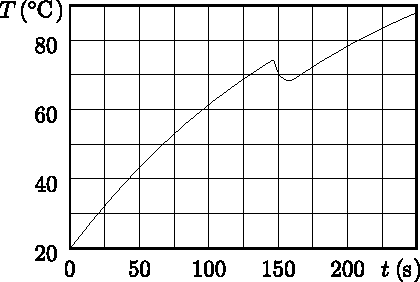
\includegraphics[width=0.7\linewidth]{2004-v3g-06-yl.pdf}
\end{center}

\hint

\solu
Vee temperatuur langeb jää sulamise tõttu. Kui jää on sulanud ja temperatuur anumas on uhtlustunud, hakkab vee temperatuur uuesti tõusma. Selleks hetkeks kui veele on antud soojushulk, mis on vajalik lisatud jää sulatamiseks, saab vee temperatuur uuesti võrdseks vee temperatuuriga enne jää lisamist. Temperatuuri $T_{1}$ juures kulub kogu kannu võimsus vee soojendamiseks, $T>T_{1}$ puhul aga tekivad vee ja toatemperatuuri erinevusest tingitud soojuskaod kannust ōhku, mistõttu vee temperatuuri kasvu kiirus aeglustub (vt. graafikut). Vee soojendamise kiirus on võrdeline $\dv{T}{t}$, s.t. graafiku tôusunurga tangensiga. Temperatuuril $\SI{70}{\degreeCelsius}$ on see vôrdne $P^{\prime}=P \tan \alpha^{\prime} / \tan \alpha$ Jooniselt leiame $\alpha \approx \num{0,5}$ ja $\alpha^{\prime} \approx \num{0,25}$, seega $P^{\prime}=\SI{500}{W}$. Samuti näeme, et vee temperatuur $T_{3}=\SI{75}{\degreeCelsius}$ taastub aja $\Delta t \approx \SI{37}{s}$ jooksul. Seega jää sulatamiseks ja temperatuurini $T_{3}$ soojendamiseks kulub soojushulk $Q=P^{\prime} \Delta t \approx \SI{18,5}{kJ}$. Jääa mass
$$
m=\frac{Q}{L+c\left(T_{3}-T_{0}\right)} \approx \SI{28}{g}.
$$

\probend
